\chapter{Hardware}
Hardware plays an important role in making a wireless sensor network low-cost and maintenance free. Designing a custom mote has advantages over using off-the-shelf motes in terms of ease of adding the energy harvesting circuit and the cost.

There are two basic strategies in designing a custom mote. First, the design could use (relatively) high-end integrated circuits, including an energy harvester, boost regulator, buck regulators, etc. The advantage of this approach is that it is easy to use integrated circuits, and the resulting circuits are small. The trade-off of this approach is that integrated circuits are expensive. Second, the design could use basic components, such as resistors, diodes, and capacitors. The advantage of this approach is a reduction in the cost of the device. The basic electronic components are less expensive than integrated circuits, and the resulting Printed Circuit Boards (PCB) are less expensive to produce. The disadvantage of this approach is that the size of the resulting circuit is typically larger. The device described in this thesis offers many of the benefits provided by devices designed using integrated circuits, except for the size. However, given that the size of the circuit is smaller than the size of our target solar panel, the circuit size is not a concern.

The hardware discussed in this thesis is a complete system, ready to be deployed in remote and hostile environments. The device is maintenance free and generates power by harvesting solar energy. The charging circuit is designed using basic electronic components, significantly reducing the cost of the device. The device works in two modes:
\begin{enumerate}
\item Solar Powered:
The device performs two tasks in solar powered mode. First, it supplies power to the circuit. Second, it charges the Li-Ion battery.
\item Battery Powered:
The circuit operates in battery powered mode whenever there is insufficient solar power. The circuit uses power from the Li-Ion battery in this mode.
\end{enumerate}

The device consists of a switching circuit which switches the circuit from solar powered mode to battery powered mode and vice-versa. The mode switches whenever the output power of the solar panel is less than the required value. The most important use of a switching circuit is to prevent power loss.

\begin{figure}[htbp]
\centering
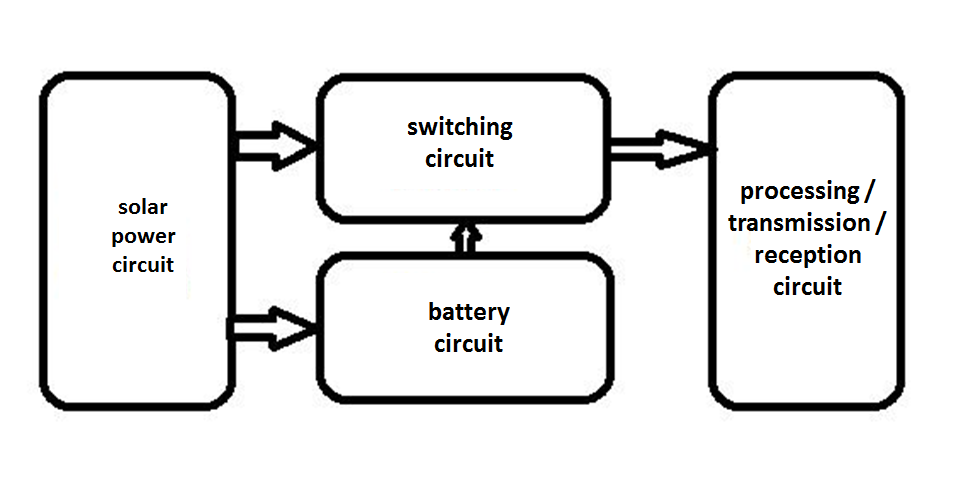
\includegraphics[width=\columnwidth]{block_dia.png}
\caption{Block Diagram of the Mote Platform}
\label{img_blockDia}
\end{figure}

The block diagram of the mote platform as shown in Figure \ref{img_blockDia} is divided into four parts:
\begin{enumerate}
\item Solar power circuit
\item Battery circuit
\item Switching circuit
\item Circuit for processing, transmission, and reception of data
\end{enumerate}

\section{Solar Power Circuit}

\begin{figure}[htbp]
\centering
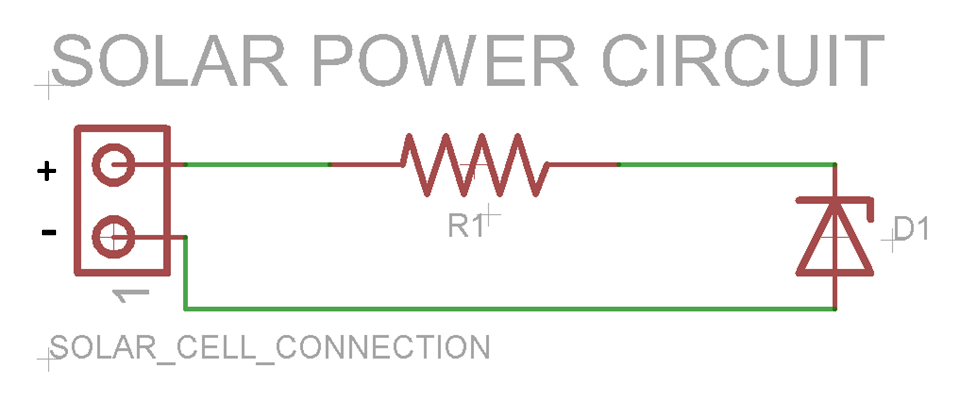
\includegraphics[width=110mm]{solar_pwr_ckt.PNG}
\caption{Solar Power Circuit}
\label{img_solarPowerCircuit}
\end{figure}

As shown in Figure \ref{img_solarPowerCircuit}, the solar power circuit consists of a 5 $volt$, 100 $mA$ solar cell, a 100 $ohm$ resistor, indicated by R1, and a 3.3 $volt$ zener diode, indicated by D1. The zener diode is connected in reverse biased mode as a voltage regulator. The zener diode ensures that the circuit receives a stable supply of 3.3 $volts$. The resistor is used as a current limiting element. It restricts the flow of current so that only a specified maximum amount of current flows through the circuit, and thus prevents the zener diode from being damaged. As shown in Figure \ref{img_solarPowerCircuit}, R1 and D1 form a voltage divider circuit, which ensures that the circuit connected parallel to the zener diode maintains a stable voltage of 3.3 $volts$ across it.% Here, we are not concerned about power loss in the resistor. since it is excess power which cannot be used to perform any useful work.

The resistance value is based on Ohm's law:
\begin{equation}
R = \frac{V_{s}-V_{z}}{I_{r}}
\end{equation}

%where,

%$R$ = Resistance($ohms$)

%$V_{s}$ = Output Voltage of solar cell($volts$)

%$V_{z}$ = Breakdown voltage of zener diode($volts$)

%$I_{r}$ = Amount of current required by circuit($mA$)

\begin{tabular}{lllp{10cm}}
where, & • & • & • \\ 
• & $R$ & = & Resistance ($ohms$) \\ 
• & $V_{s}$ & = & Output voltage of solar cell ($volts$) \\ 
• & $V_{z}$ & = & Breakdown voltage of zener diode ($volts$) \\ 
• & $I_{r}$ & = & Amount of current required by circuit ($mA$) \\ 
 &  &  &  \\ 
\end{tabular} 


The solar power circuit performs two functions.
\begin{enumerate}
\item Provide the voltage and current required by the processing circuit.
\item Provide the excess current to the battery circuit to charge the battery.
\end{enumerate}

\section{Battery Circuit}

\begin{figure}[htbp]
\centering
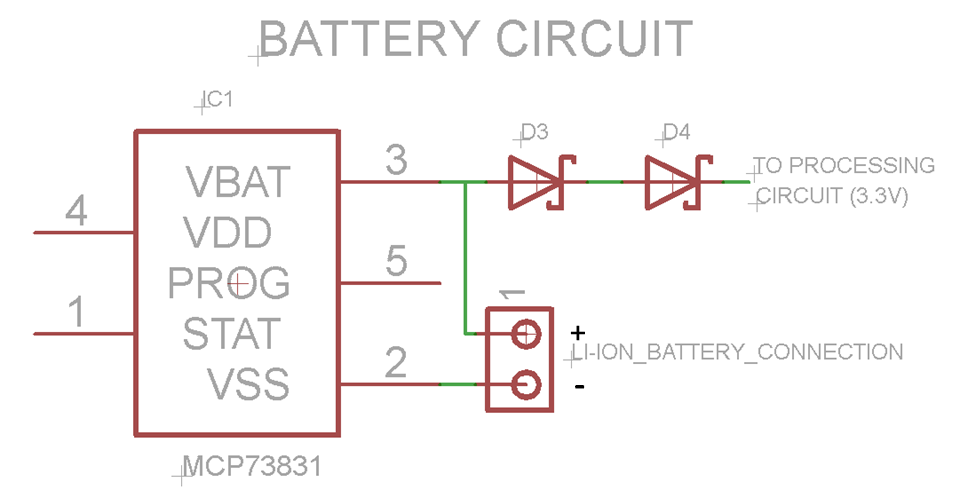
\includegraphics[width=\columnwidth]{battery_ckt.PNG}
\caption{Battery Circuit}
\label{img_batteryCircuit}
\end{figure}

As shown in Figure \ref{img_batteryCircuit}, the battery circuit consists of an MCP73831 integrated circuit, an 850 $mAh$ Li-Ion battery, and two Schottky diodes \cite{bib_diode}, indicated in Figure \ref{img_batteryCircuit} as D3 and D4. The MCP73831 is used to charge the Li-Ion battery. Schottky diodes are usually used for fast switching of inputs, as their response time is faster, and their forward voltage drop is less than normal diodes. The Schottky diode has a low forward voltage drop of only 0.2 $volts$ and a high reverse breakdown voltage of 15 $volts$. In this circuit, we use the low forward voltage drop property of the Schottky diode to reduce the voltage. According to the discharge curve of the Li-Ion battery \cite{bib_battery}, the output voltage of the battery is fairly stable at 3.7 $volts$. The processing circuit operates properly at 3.3 $volts$. This voltage drop is provided by the diodes. As shown in Figure \ref{img_circuit}, if solar energy is not available, voltage at the cathode of diode D4 is less than the voltage at its anode. This makes diode D4 forward biased, and hence the circuit runs on battery power. If solar energy is available, and the output voltage of the battery is less than or equal to 3.7 $volts$, these diodes become reverse biased as voltage at the cathode of the Schottky diode is more than the voltage at the anode, and hence the circuit runs only on solar power while the battery charges. This helps conserve the battery whenever solar energy is available.

% ask Jason whether to mention about resistor or not to provide the voltage drop in place of diode and its disadvantage

The lifetime of a Li-Ion battery is directly proportional to how the battery is charged. There are three charging stages:

\begin{enumerate}
\item Precondition charging
\item Constant current charging
\item Constant voltage charging
\end{enumerate}

Depending on the state and capacity of the battery, we must decide on the maximum charging current that will not damage the battery. Li-Ion batteries are very sensitive to charging voltage; the charging voltage should not exceed 1.19\% of the rated value. To ensure the charging voltage is within an acceptable range, the circuit uses a MCP73831 \cite{bib_mcp73831} integrated circuit instead of basic electronic components. MCP73831 determines the charging stage of the battery. The MCP73831 is also fairly inexpensive (0.69 USD).%Another benefit of using the MCP73831 rather than basic electronic components, is the MCP73831 is less expensive.
%To overcome this problem, the circuit uses a MCP73831 \cite{bib_mcp73831} integrated circuit. The main reason to use MCP73831 in place of basic electronic components is the sensitivity of the Li-Ion battery towards charging voltage. Further, designing a Li-Ion battery charging circuit using basic electronic components is more expensive than MCP73831 integrated circuit.

\section{Switching Circuit}

\begin{figure}[htbp]
\centering
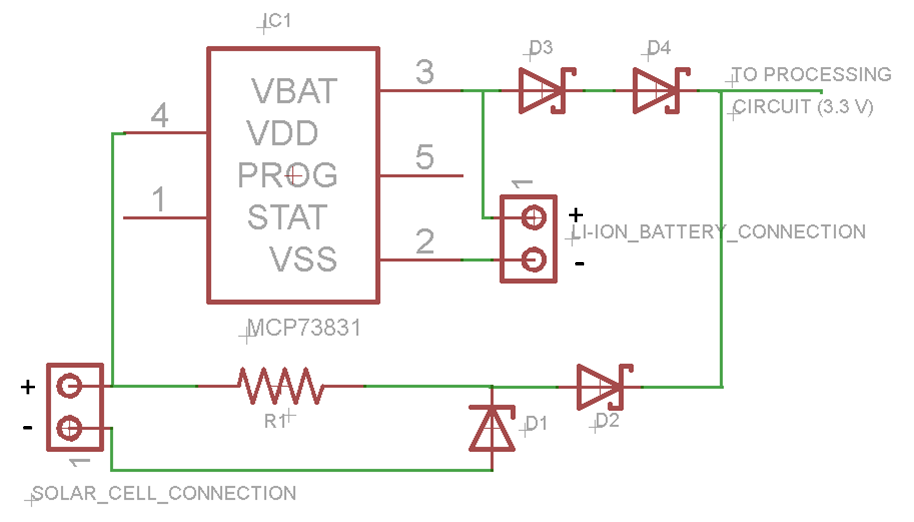
\includegraphics[width=\columnwidth]{correct_ckt.PNG}
\caption{Complete Circuit Diagram}
\label{img_circuit}
\end{figure}

\begin{figure}[htbp]
\centering

\includegraphics[width=110mm]{switchin_ckt.PNG}
\caption{Switching Circuit}
\label{img_switchingCircuit}
\end{figure}

Figure \ref{img_switchingCircuit} shows the switching circuit, which consists of a Schottky diode, indicated by D2. The Schottky diode is highly suitable for our application. Consider the situation when it is night; the solar panel will not source power; instead, it will sink power. If the Schottky diode shown in Figure \ref{img_circuit} as D2 is not present, the zener diode denoted as D1 will connect to the battery and it will continuously consume power from the battery, resulting in battery failure. In this situation, the Schottky diode D2 becomes reverse biased, resulting in high reverse breakdown voltage, causing the path between the battery circuit and solar power circuit to become (effectively) an open circuit, resulting in savings in battery power.


\section{Circuit for Processing, Transmission and Reception of Data}
This section describes the processing and transmission circuit, and the connection of the \textit{\textbf{root}} mote with the \textit{base station}. The processing circuit consists of an ATMEGA168 microcontroller \cite{bib_atmega}, and a radio frequency transceiver, the RFM12 \cite{bib_rfm12}. The RFM12 transmits and receives data. It offers many advantages over more costly radios, such as the CC2420, the CC2400, and others, including programmable variable data transmission rates, variable channel frequency, and most importantly, low power consumption and cost. The ATMEGA168 is used to sense and process data \textit{in situ}. The ATMEGA168 transmits the processed data using the RFM12 transceiver to the neighboring motes. If the mote is the  \textit{\textbf{root}}, it transmits the data to the base station using an FT232R \cite{bib_ftdi} chip, a UART to USB converter. The base station runs Python code that processes, analyzes, and stores the data.

The main motivation for creating this design and not using off-the-shelf hardware, such as the TelosB mote \cite{bib_telob}, is the hardware cost and the ease of adding the harvesting circuit. This thesis focuses on making an inexpensive network that provides all the basic functionality of off-the-shelf motes. Table \ref{table_costOfComponents} shows the cost of the individual components used to make the device, as well as the costs when the components are purchased in volume.

\begin{table}[htbp]
\begin{center}
\begin{tabular}{|l||c|c|c|}
\hline 
 & \multicolumn{3}{ |c| }{\textbf{Quantity}} \\
\hline 
\hline 
\textbf{Components} & \textbf{1} & \textbf{100} & \textbf{1000} \\ 
\hline 
\hline 
Solar Panel & 6.90 & 5.50 & 5.50 \\ 
\hline 
Li-Ion battery  & 11.61 & 3.87 & 3.22 \\ 
\hline 
RFM12 & 6.95 & 5.56 & 5.56 \\ 
\hline 
ATMEGA168 & 2.43 & 1.35 & 1.35 \\ 
\hline 
MCP73831 & 0.68 & 0.42 & 0.42 \\ 
\hline 
Resistor, Capacitor, and Diodes & 2.97 & 1.59 & 0.88 \\ 
\hline 
% &  &  &  \\ 
\hline 
Total & 31.54 & 18.29 & 16.93 \\ 
\hline 
Cost of 1 unit & 31.54 &  &  \\ 
\hline 
Cost of 100 units &  & 1829.00 &  \\ 
\hline 
Cost of 1000 units &  &  & 16930.00 \\ 
\hline 
\end{tabular} 
\end{center}
\caption{Cost of Components (in USD) \cite{bib_cost}}
\label{table_costOfComponents}
\end{table}

\begin{figure}[htbp]
\centering
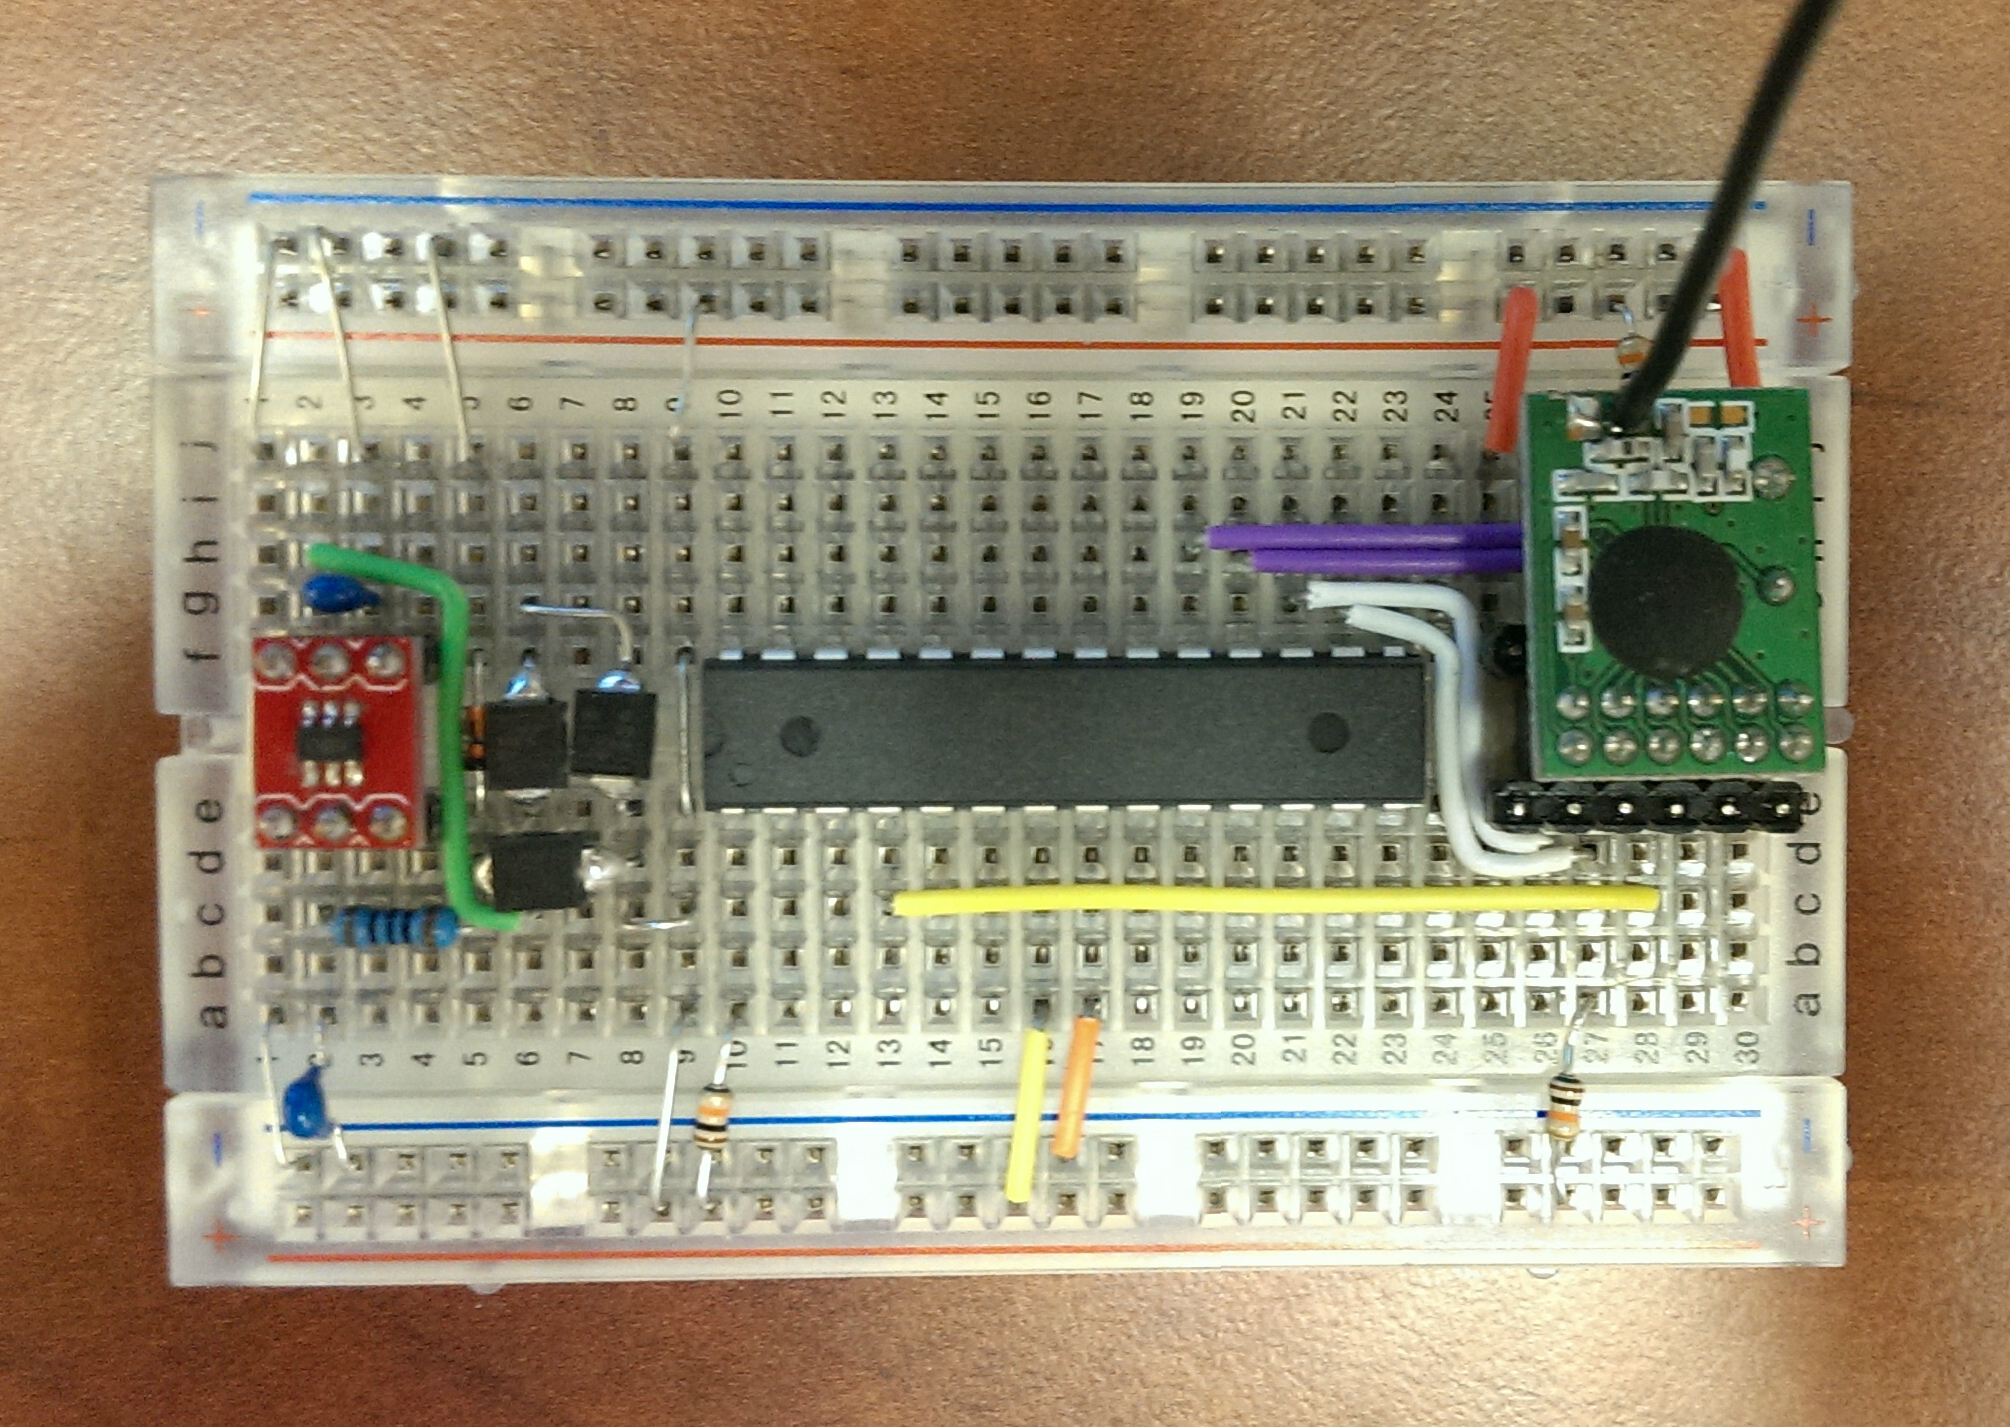
\includegraphics[width=110mm]{prototype.jpg}
\caption{Prototype Board}
\label{img_prototypeBoard}
\end{figure}

The prototype of the board is shown in Figure \ref{img_prototypeBoard}. The prototype board consists of a MCP73831 Li-Ion battery charger, Schottky diodes, an ATMEGA168 microcontroller to process data, and an RFM12 transceiver to transmit and receive data from other motes. In the future, the prototype board can be converted to a PCB to further reduce the size of the circuit. This circuit can be built on a PCB that is 1 square inch.
%This circuit can be built on 1 X 1 inch of square using PCB. 

\begin{figure}[htbp]
\centering
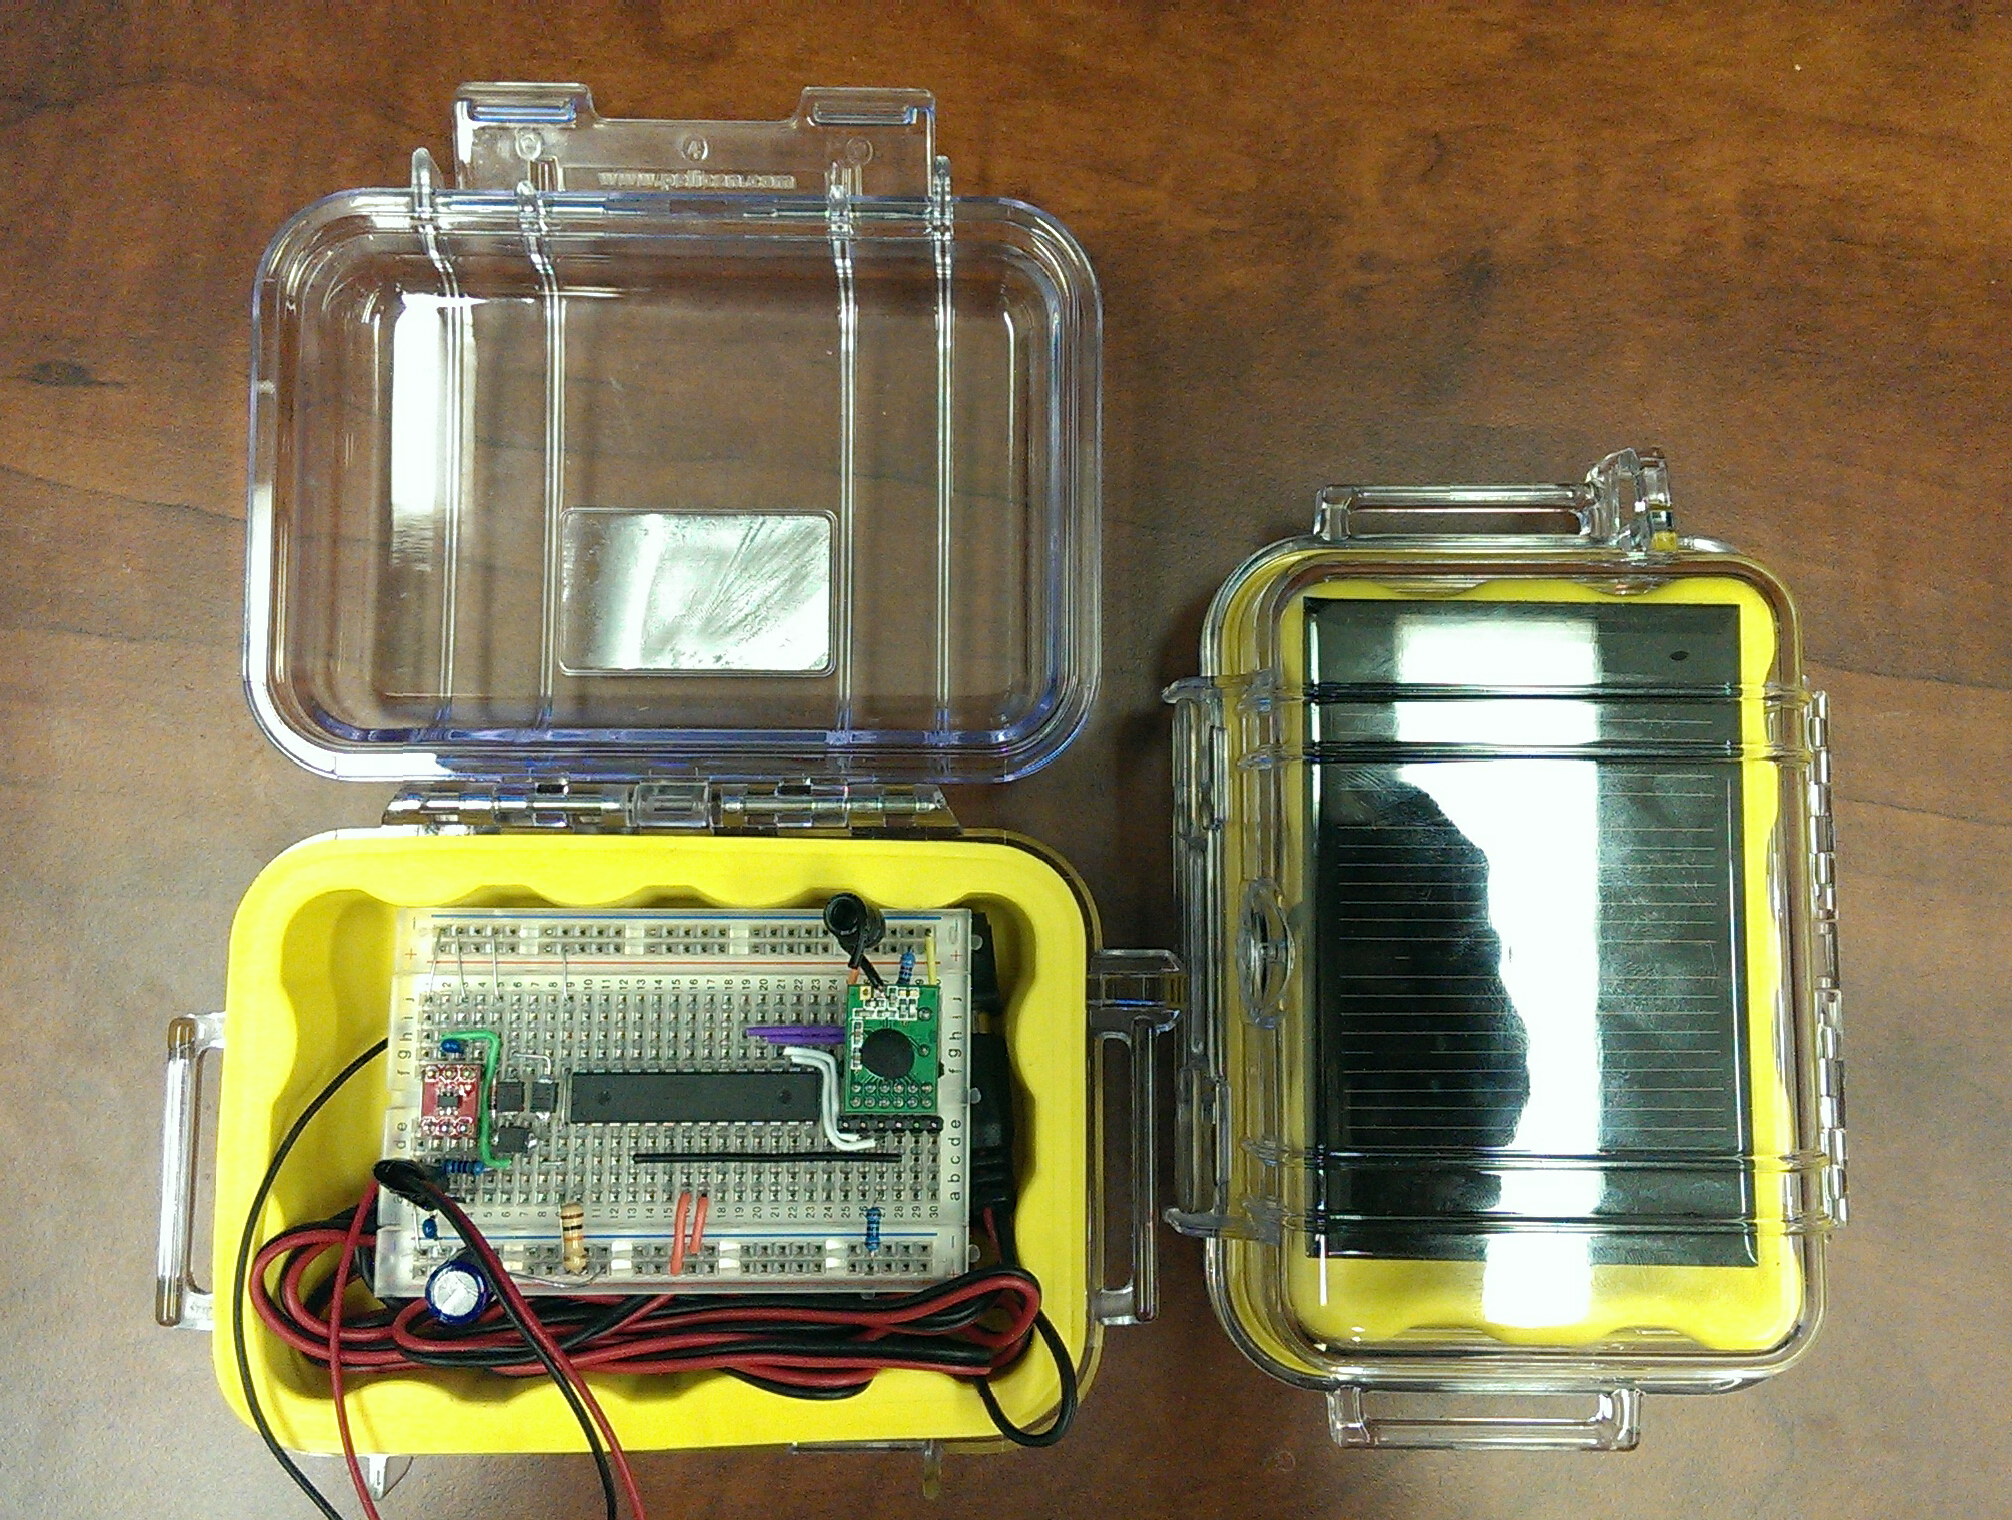
\includegraphics[width=110mm]{box_ckt.jpg}
\caption{Safety Enclosure}
\label{img_boxCircuit}
\end{figure}

As shown in Figure \ref{img_boxCircuit}, the circuit is then enclosed in a plastic container to prevent it from being damaged by environmental factors like rain or dust. Figure \ref{img_boxCircuit} shows the prototype board and the solar panel enclosed in the plastic container.
